\chapter{Organização funcional de uma planta com flores}\label{ch:b1:flowering-plant-organization}

Um carvalho de dois séculos está no mesmo metro quadrado de solo em que
germinou. Ele nunca comeu, nunca se moveu, nunca manteve a própria
temperatura; e ainda assim construiu quarenta toneladas de madeira, e
todo verão espalha quinhentos metros quadrados de \omterm{def:b1:flowering-plant-organization:organs}{folha} pelo ar e uma
superfície ainda maior de \omterm{def:b1:flowering-plant-organization:organs}{raiz} pelo solo. Uma planta com flores é a
outra resposta ao problema do \cref{ch:b1:organism-environment}: um
autótrofo fixo que encontra o ambiente não interiorizando as trocas
dele, e sim fazendo as próprias \omterm{prop:b1:organism-environment:surfaces}{superfícies de troca} crescerem para
fora, indefinidamente, onde quer que estejam a luz e a água. Este
capítulo descreve como um corpo desses é organizado --- os \omterm{def:b1:mammal-organization:organ}{órgãos} dele,
os tecidos, as superfícies que ele desdobra e o crescimento que as
constrói.

\begin{omfigure}
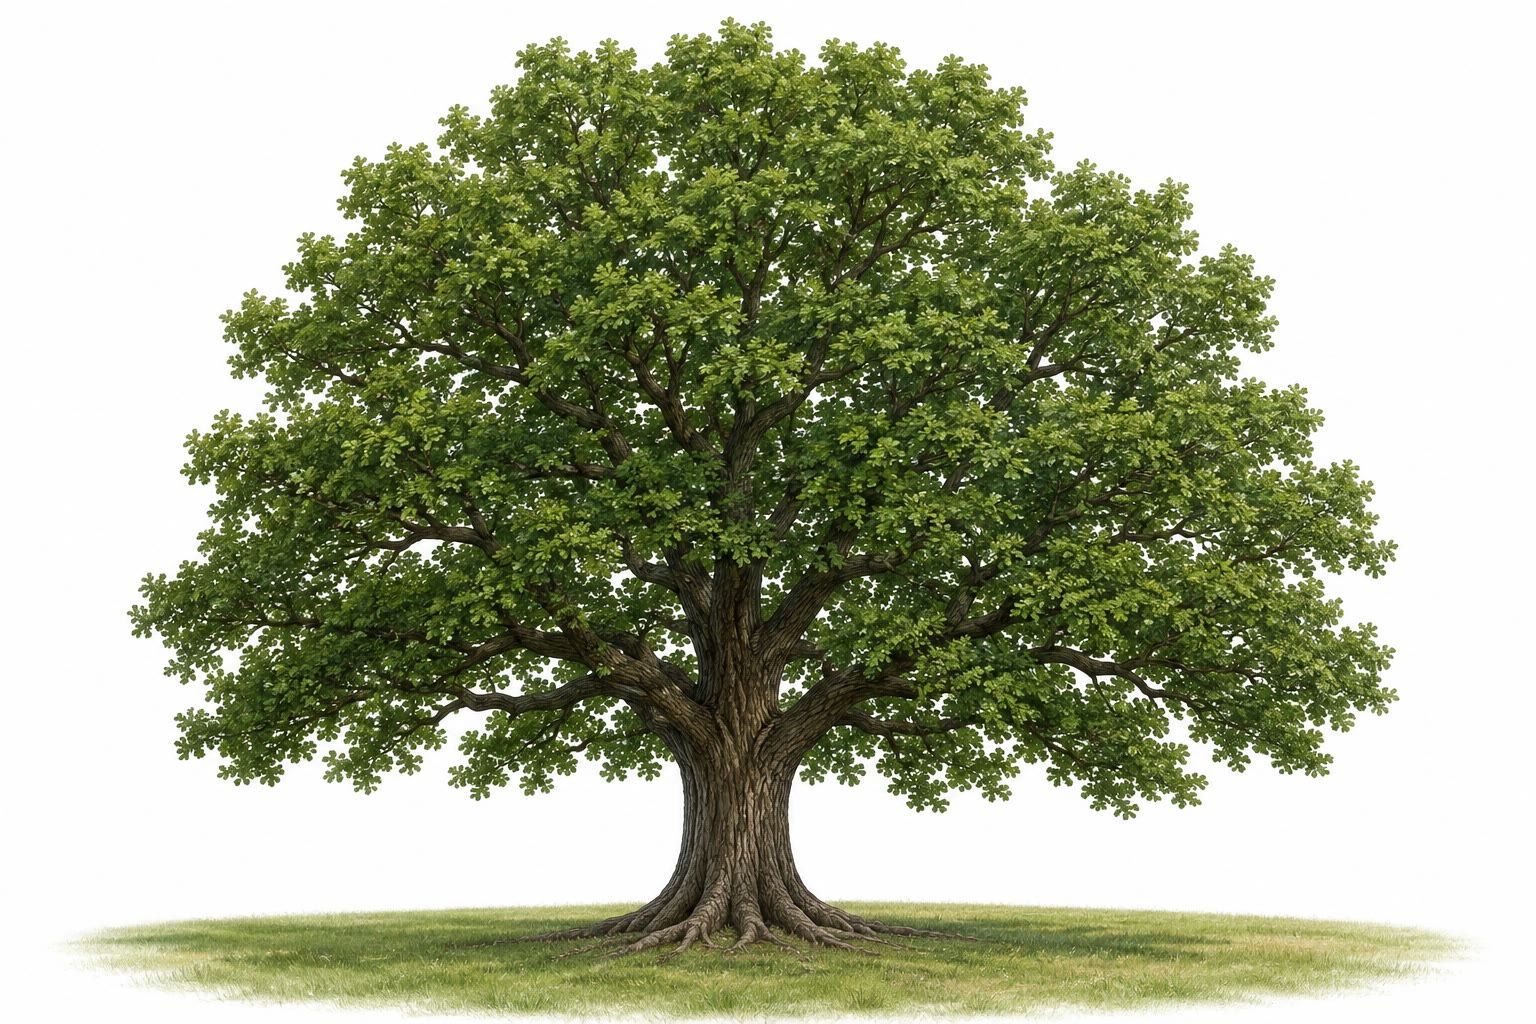
\includegraphics[width=0.62\linewidth]{images/book3/ai/b3-03-oak-tree.jpg}

{\small Um carvalho solitário no verão. A copa dele é um arranjo de
\omterm{def:b1:flowering-plant-organization:organs}{folhas} espalhadas para interceptar a luz; o sistema radicular sob a
grama é tão largo quanto a copa e a superfície dele, várias vezes maior.}
\end{omfigure}

\section{O corpo vegetativo}

\begin{definition}[Raiz, caule, folha]\label{def:b1:flowering-plant-organization:organs}
O corpo vegetativo de uma planta com flores é feito de três tipos de
\omterm{def:b1:mammal-organization:organ}{órgão}. A \emph{raiz}\index{raiz} fixa a planta e absorve água e íons
minerais do solo; ela cresce pela ponta, ramifica-se e carrega
\emph{pelos radiculares}\index{pelo radicular} logo atrás da ponta. O
\emph{caule}\index{caule} leva as folhas em direção à luz e conduz entre
raízes e folhas; ele é construído a partir de unidades repetidas, cada
uma um \emph{nó}\index{nó} que carrega uma folha e uma gema axilar, e um
\emph{entrenó}\index{entrenó} entre dois nós. A
\emph{folha}\index{folha} é o \omterm{def:b1:mammal-organization:organ}{órgão} da fotossíntese: uma lâmina achatada
de superfície grande e espessura pequena, sustentada por um pecíolo. As
raízes formam o sistema radicular; os caules e as folhas, a parte aérea.
\end{definition}

\begin{proposition}[Um corpo modular e aberto]\label{prop:b1:flowering-plant-organization:modular}
O corpo da planta é \emph{modular}\index{crescimento modular}: a parte
aérea é uma série de unidades idênticas (\omterm{def:b1:flowering-plant-organization:organs}{nó}, \omterm{def:b1:flowering-plant-organization:organs}{folha}, gema, \omterm{def:b1:flowering-plant-organization:organs}{entrenó})
acrescentadas uma após a outra por uma gema apical, e cada gema axilar
pode iniciar uma nova série. O crescimento é
\emph{indeterminado}\index{crescimento indeterminado}: não há tamanho
adulto, e a planta continua acrescentando módulos, e portanto
superfície, enquanto viver. O número e a posição dos módulos dependem do
local --- luz, água, danos ---, de modo que a mesma espécie assume
formas diferentes em lugares diferentes. O corpo de um mamífero, ao
contrário, é fechado: os \omterm{def:b1:mammal-organization:organ}{órgãos} dele são fixos em número e ele para de
crescer num tamanho determinado.
\end{proposition}

\begin{omfigure}
\begin{tikzpicture}[font=\small, >=Stealth, line cap=round]
  % stem axis
  \draw[very thick, omExo!70!black] (0,0) -- (0,6.2);
  \node[circle, fill=omExo!70!black, inner sep=2.2pt] at (0,6.2) {};
  \node[right, font=\footnotesize, align=left] at (0.25,6.35) {gema apical: acrescenta\\ novos módulos acima};
  % nodes with leaves and axillary buds
  \foreach \y/\side in {1.2/1, 2.6/-1, 4.0/1, 5.2/-1} {
    \fill[omExo!70!black] (0,\y) circle (2pt);
    \draw[thick, omExo!70!black] (0,\y) -- (\side*0.6,\y+0.25);
    \draw[thick, omExo, fill=omExo!30] (\side*0.6,\y+0.25) .. controls (\side*1.4,\y+0.6) and (\side*2.2,\y+0.15) .. (\side*2.0,\y-0.1) .. controls (\side*1.4,\y-0.25) and (\side*0.9,\y-0.05) .. (\side*0.6,\y+0.25);
    \fill[omProp] (\side*0.18,\y+0.28) circle (2pt);
  }
  % module bracket
  \draw[thick, gray] (-2.4,1.2) -- (-2.6,1.2) -- (-2.6,2.6) -- (-2.4,2.6);
  \node[left, font=\footnotesize, align=right, gray] at (-2.65,1.9) {um módulo:\\ entrenó, nó,\\ folha, gema axilar};
  \node[right, font=\footnotesize] at (2.2,4.1) {folha};
  \node[right, font=\footnotesize, omProp] at (0.25,2.95) {gema axilar};
  \node[left, font=\footnotesize] at (-0.3,3.3) {entrenó};
  \node[left, font=\footnotesize] at (-0.3,3.98) {nó};
  % roots
  \draw[very thick, omDef!70!black] (0,0) -- (0,-1.6);
  \draw[thick, omDef!70!black] (0,-0.5) -- (-1.0,-1.3) (0,-0.9) -- (0.9,-1.5) (0,-1.2) -- (-0.5,-2.0);
  \foreach \x in {-0.12,-0.06,0.06,0.12} \draw[omDef!70!black] (\x,-1.55) -- (\x*3,-1.9);
  \node[right, font=\footnotesize, align=left] at (0.5,-0.75) {sistema radicular: cresce pelas\\ pontas, com pelos radiculares atrás};
  \draw[dashed, gray] (-3.0,0) -- (3.2,0);
  \node[font=\footnotesize, gray, anchor=south east] at (3.2,0.02) {superfície do solo};
\end{tikzpicture}

{\small A parte aérea como uma pilha de módulos. Cada \omterm{def:b1:flowering-plant-organization:organs}{nó} carrega uma
\omterm{def:b1:flowering-plant-organization:organs}{folha} e uma gema axilar; a gema apical acrescenta módulos acima, e
qualquer gema axilar pode iniciar um ramo. O sistema radicular cresce
pelas pontas.}
\end{omfigure}

\section{Os tecidos do corpo primário}

\begin{definition}[Tecidos de revestimento, fundamental e vascular]\label{def:b1:flowering-plant-organization:tissues}
Todo \omterm{def:b1:mammal-organization:organ}{órgão} da planta é construído a partir de três sistemas de tecidos.
O \emph{tecido de revestimento}\index{tecido de revestimento} é a
\emph{epiderme}\index{epiderme}, uma única camada de células que recobre
o \omterm{def:b1:mammal-organization:organ}{órgão}, revestida no ar por uma \emph{cutícula}\index{cutícula} cerosa
e perfurada por \emph{estômatos}\index{estômato}, e prolongada na \omterm{def:b1:flowering-plant-organization:organs}{raiz}
pelos \omterm{def:b1:flowering-plant-organization:organs}{pelos radiculares}. O
\emph{tecido fundamental}\index{tecido fundamental} preenche o \omterm{def:b1:mammal-organization:organ}{órgão}: o
\emph{parênquima}\index{parênquima} (células vivas de parede fina, para
a fotossíntese e o armazenamento), o
\emph{colênquima}\index{colênquima} (células vivas com paredes
espessadas de modo desigual, o sustento flexível dos \omterm{def:b1:flowering-plant-organization:organs}{caules} jovens) e o
\emph{esclerênquima}\index{esclerênquima} (células de paredes espessas e
lignificadas, mortas na maturidade, o sustento rígido: fibras e
esclereídes). O \emph{tecido vascular}\index{tecido vascular} conduz: o
\emph{xilema}\index{xilema} leva água e minerais para cima nos
\emph{traqueídes}\index{traqueíde} e \emph{vasos}\index{vaso} ocos,
lignificados e mortos (\cref{ch:b1:plant-transport}); o
\emph{floema}\index{floema} leva açúcares nos
\emph{tubos crivados}\index{tubo crivado} vivos, mantidos vivos pelas
células companheiras deles.
\end{definition}

\begin{omfigure}
\begin{tikzpicture}
  \node[anchor=south west, inner sep=0] (img) at (0,0)
    {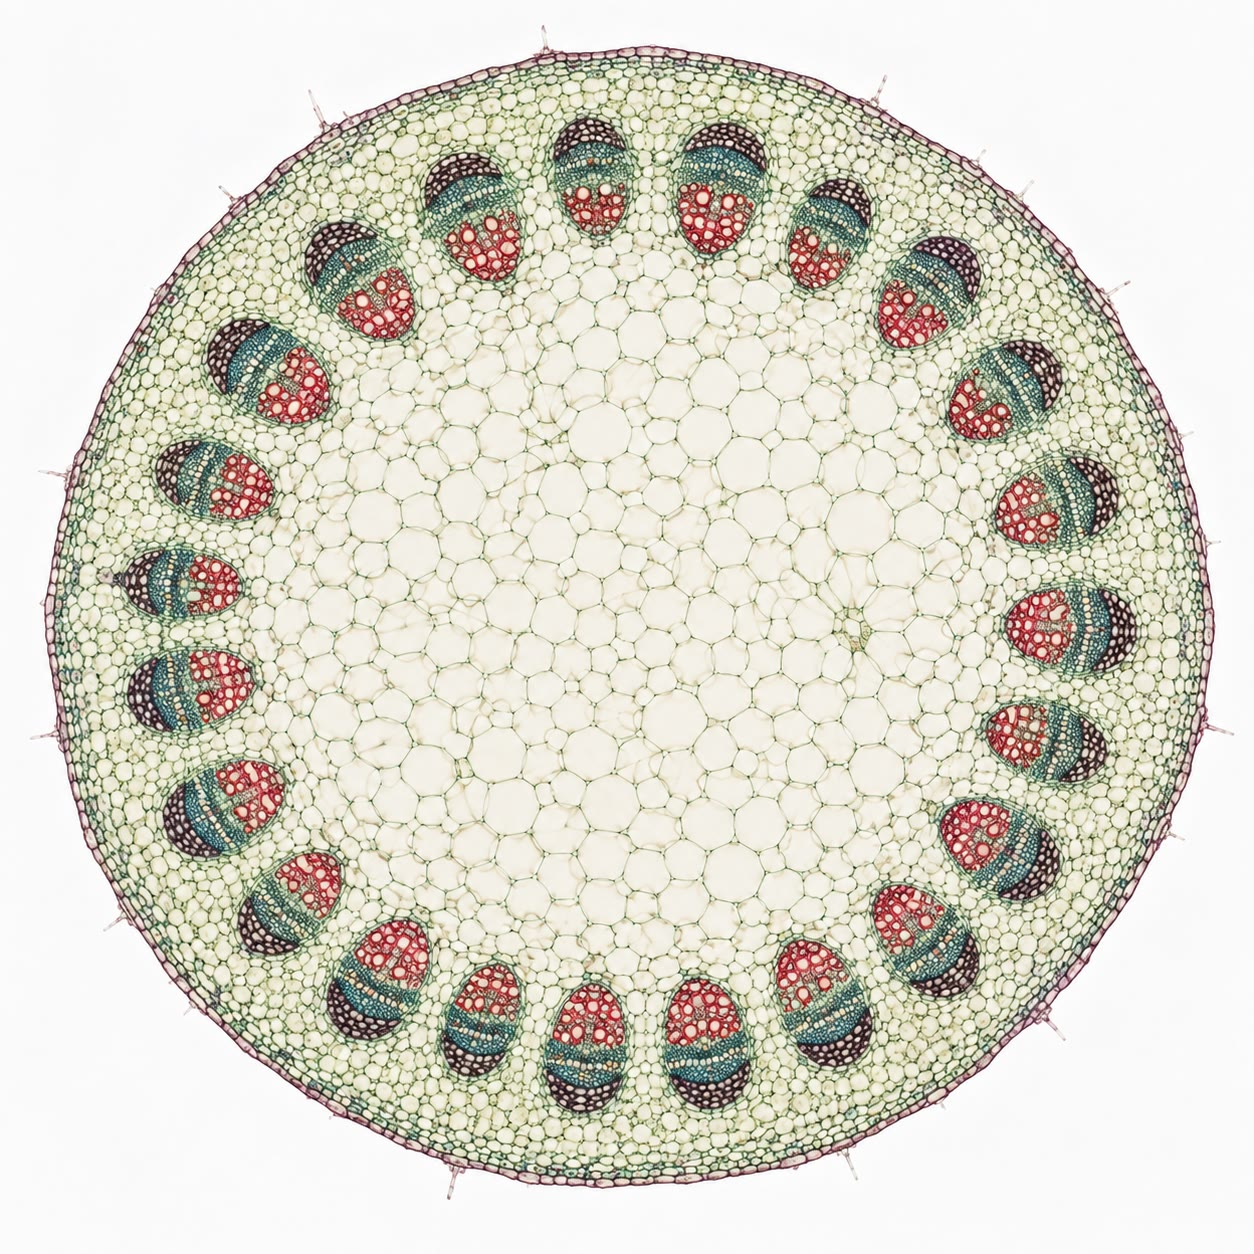
\includegraphics[width=0.5\linewidth]{images/book3/ai/fig-dicot-stem-cross.jpg}};
  \begin{scope}[x={(img.south east)}, y={(img.north west)},
      every node/.style={font=\small}]
    \draw[omDef, thick] (0.50,0.895) -- (0.50,1.06) node[above] {calota de esclerênquima de um feixe};
    \draw[omDef, thick] (0.87,0.50) -- (1.03,0.60) node[right] {floema (para fora)};
    \draw[omDef, thick] (0.81,0.50) -- (1.03,0.42) node[right] {xilema (para dentro)};
    \draw[omDef, thick] (0.50,0.50) -- (-0.03,0.50) node[left] {medula};
    \draw[omDef, thick] (0.085,0.56) -- (-0.03,0.66) node[left] {córtex};
    \draw[omDef, thick] (0.06,0.40) -- (-0.03,0.32) node[left] {epiderme};
  \end{scope}
\end{tikzpicture}

{\small Corte transversal de um \omterm{def:b1:flowering-plant-organization:organs}{caule} jovem de dicotiledônea. Os feixes
vasculares formam um anel: em cada um, o \omterm{def:b1:flowering-plant-organization:tissues}{xilema} (corado de vermelho,
lignificado) fica voltado para o centro e o \omterm{def:b1:flowering-plant-organization:tissues}{floema} para fora, sob uma
calota de fibras. Dentro do anel, a medula; fora dele, o córtex e a
epiderme.}
\end{omfigure}

\begin{omfigure}
\begin{tikzpicture}
  \node[anchor=south west, inner sep=0] (img) at (0,0)
    {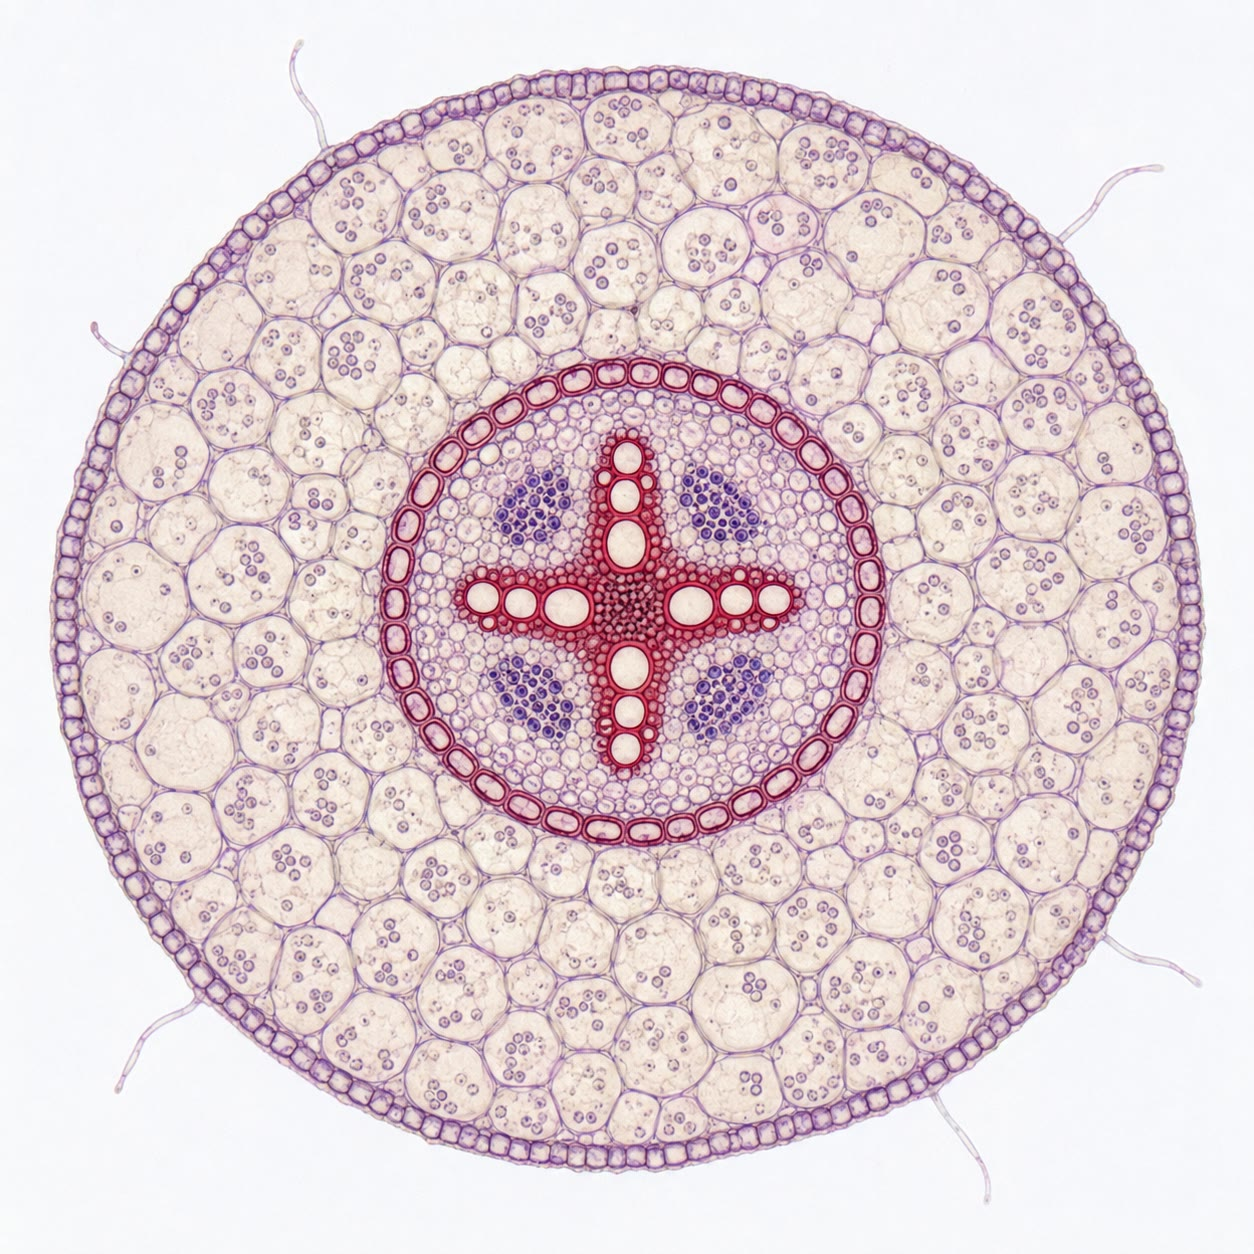
\includegraphics[width=0.46\linewidth]{images/book3/ai/fig-root-cross.jpg}};
  \begin{scope}[x={(img.south east)}, y={(img.north west)},
      every node/.style={font=\small}]
    \draw[omDef, thick] (0.50,0.52) -- (0.50,1.06) node[above] {estrela central de xilema};
    \draw[omDef, thick] (0.58,0.45) -- (1.03,0.38) node[right] {floema entre os braços};
    \draw[omDef, thick] (0.695,0.50) -- (1.03,0.58) node[right] {endoderme};
    \draw[omDef, thick] (0.30,0.50) -- (-0.03,0.50) node[left] {córtex};
    \draw[omDef, thick] (0.06,0.62) -- (-0.03,0.74) node[left] {epiderme e pelos radiculares};
  \end{scope}
\end{tikzpicture}

{\small Corte transversal de uma \omterm{def:b1:flowering-plant-organization:organs}{raiz} jovem de dicotiledônea. Um único
cilindro vascular central: uma estrela de \omterm{def:b1:flowering-plant-organization:tissues}{xilema} com \omterm{def:b1:flowering-plant-organization:tissues}{floema} nos ângulos,
delimitada pela \omterm{prop:b1:flowering-plant-organization:stemroot}{endoderme}; em volta dela um córtex largo; por fora, a
epiderme, que carrega \omterm{def:b1:flowering-plant-organization:organs}{pelos radiculares}.}
\end{omfigure}

\begin{proposition}[Caule e raiz diferem na posição dos tecidos vasculares]\label{prop:b1:flowering-plant-organization:stemroot}
No \omterm{def:b1:flowering-plant-organization:organs}{caule} jovem os \omterm{def:b1:flowering-plant-organization:tissues}{tecidos vasculares} formam feixes dispostos em anel
(dicotiledôneas) ou espalhados pelo \omterm{def:b1:flowering-plant-organization:tissues}{tecido fundamental}
(monocotiledôneas), cada feixe com o \omterm{def:b1:flowering-plant-organization:tissues}{xilema} voltado para o centro e o
\omterm{def:b1:flowering-plant-organization:tissues}{floema} para fora; não há \omterm{prop:b1:flowering-plant-organization:stemroot}{endoderme}, e o \omterm{def:b1:flowering-plant-organization:tissues}{tecido fundamental} está dividido
em uma medula central e um córtex externo. Na \omterm{def:b1:flowering-plant-organization:organs}{raiz} jovem há um único
cilindro central: o \omterm{def:b1:flowering-plant-organization:tissues}{xilema} forma uma estrela (de dois a cinco braços nas
dicotiledôneas, muitos nas monocotiledôneas), o \omterm{def:b1:flowering-plant-organization:tissues}{floema} fica entre os
braços, e o cilindro é delimitado pela \emph{endoderme}\index{endoderme},
um anel de células cujas paredes radiais levam uma faixa impermeável
(\cref{ch:b1:plant-water-minerals}). A posição corresponde à função: um
\omterm{def:b1:flowering-plant-organization:organs}{caule} resiste à flexão, e um anel de feixes perto da superfície dele é o
arranjo mais rígido para a sua massa; uma \omterm{def:b1:flowering-plant-organization:organs}{raiz} resiste à tração, e um
cilindro central é o arranjo de um cabo.
\end{proposition}

\begin{method}[Identificar um corte de planta]\label{met:b1:flowering-plant-organization:section}
\begin{enumerate}
  \item Um único cilindro vascular central com \omterm{prop:b1:flowering-plant-organization:stemroot}{endoderme}: uma \omterm{def:b1:flowering-plant-organization:organs}{raiz}.
        Feixes em anel ou espalhados, com medula: um \omterm{def:b1:flowering-plant-organization:organs}{caule}. Um \omterm{def:b1:mammal-organization:organ}{órgão}
        achatado com duas epidermes e uma camada lacunosa: uma \omterm{def:b1:flowering-plant-organization:organs}{folha}.
  \item \omterm{def:b1:flowering-plant-organization:organs}{Raiz} com poucos braços de \omterm{def:b1:flowering-plant-organization:tissues}{xilema} (2--5): dicotiledônea; muitos
        braços em torno de uma medula: monocotiledônea. \omterm{def:b1:flowering-plant-organization:organs}{Caule} com feixes
        em um só anel: dicotiledônea; feixes espalhados:
        monocotiledônea.
  \item O \omterm{def:b1:flowering-plant-organization:tissues}{xilema} é reconhecido pelas células grandes, de parede espessa
        e vazias (vermelhas com os corantes usuais); o \omterm{def:b1:flowering-plant-organization:tissues}{floema}, pelas
        células vivas pequenas, com \omterm{def:b1:flowering-plant-organization:tissues}{tubos crivados} e células
        companheiras (verdes ou azuis).
  \item Num corte de \omterm{def:b1:flowering-plant-organization:organs}{caule}, o \omterm{def:b1:flowering-plant-organization:tissues}{xilema} aponta para dentro e o \omterm{def:b1:flowering-plant-organization:tissues}{floema} para
        fora. Numa \omterm{def:b1:flowering-plant-organization:organs}{raiz}, \omterm{def:b1:flowering-plant-organization:tissues}{xilema} e \omterm{def:b1:flowering-plant-organization:tissues}{floema} se alternam sobre o mesmo raio.
\end{enumerate}
\end{method}

\begin{omfigure}
\begin{tikzpicture}
  \node[anchor=south west, inner sep=0] (img) at (0,0)
    {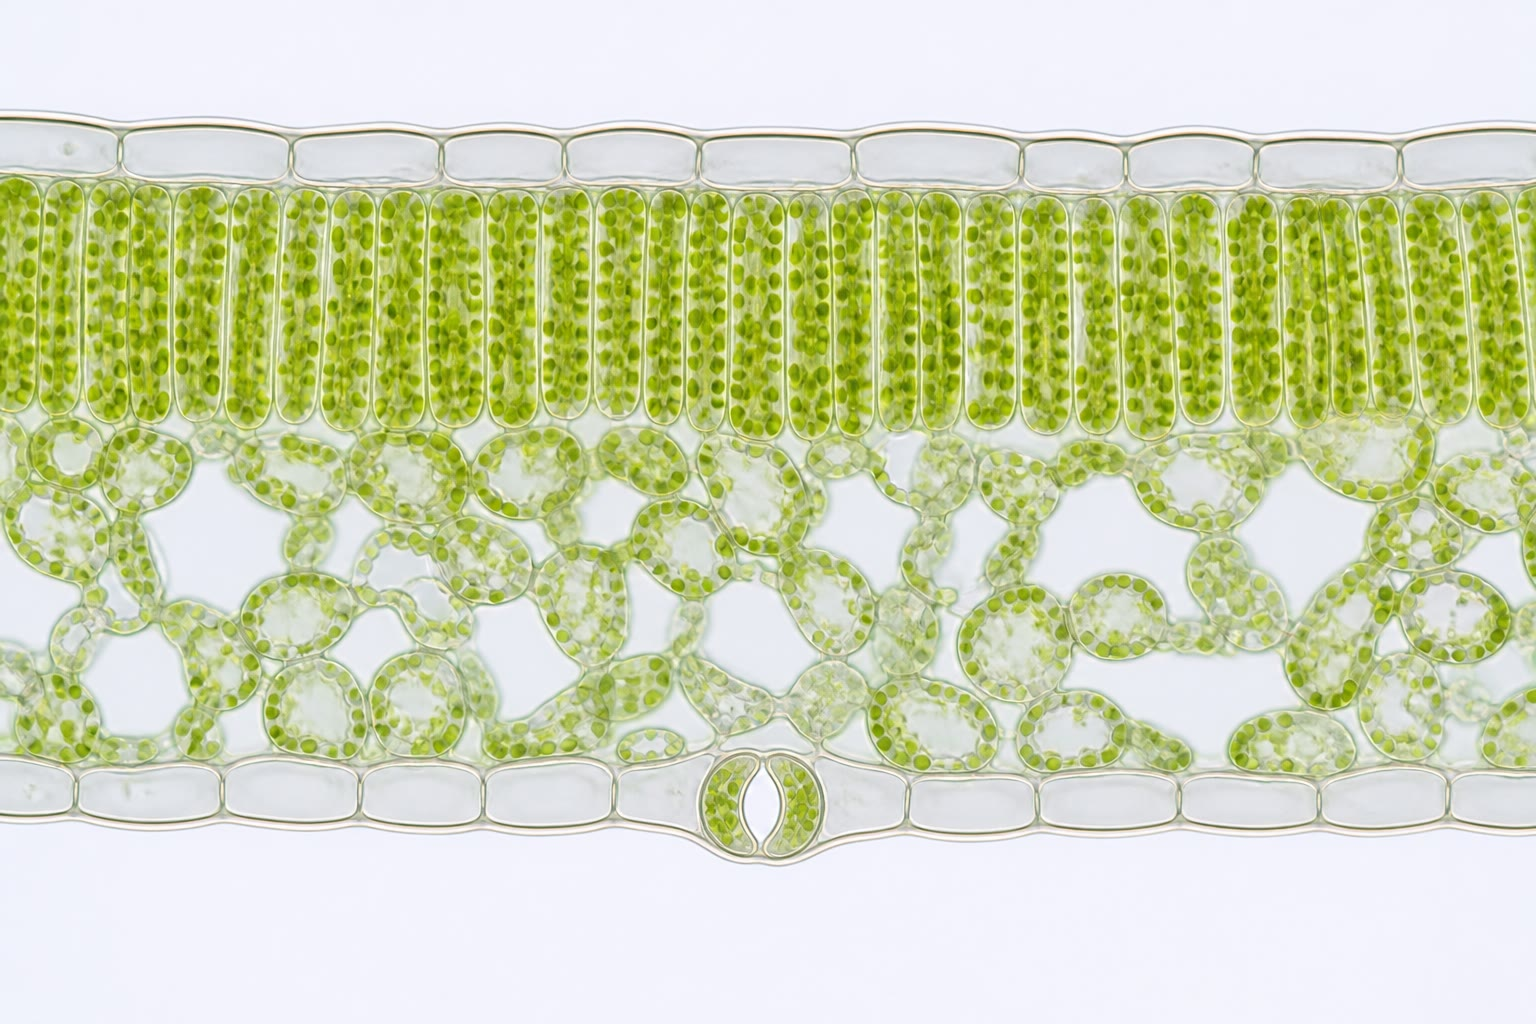
\includegraphics[width=0.48\linewidth]{images/book2/ai/fig-leaf-cross-section.jpg}};
  \begin{scope}[x={(img.south east)}, y={(img.north west)},
      every node/.style={font=\small}]
    \draw[omDef, thick] (0.50,0.94) -- (0.50,1.08) node[above] {epiderme superior, cutícula};
    \draw[omDef, thick] (0.30,0.70) -- (-0.03,0.80) node[left] {parênquima paliçádico};
    \draw[omDef, thick] (0.30,0.35) -- (-0.03,0.30) node[left] {parênquima lacunoso};
    \draw[omDef, thick] (0.70,0.50) -- (1.03,0.60) node[right] {nervura};
    \draw[omDef, thick] (0.60,0.10) -- (1.03,0.10) node[right] {estômato};
  \end{scope}
\end{tikzpicture}

{\small Corte transversal de uma \omterm{def:b1:flowering-plant-organization:organs}{folha}. Entre as duas epidermes, as
células paliçádicas colunares repletas de cloroplastos ficam voltadas
para a luz, e as células lacunosas frouxas de baixo deixam espaços de ar
que se abrem pelos \omterm{def:b1:flowering-plant-organization:tissues}{estômatos}. As nervuras trazem a água e levam o
açúcar.}
\end{omfigure}

\begin{example}[Onde acontecem as trocas]\label{ex:b1:flowering-plant-organization:where}
O dióxido de carbono entra numa \omterm{def:b1:flowering-plant-organization:organs}{folha} pelos \omterm{def:b1:flowering-plant-organization:tissues}{estômatos}, atravessa os
espaços de ar da camada lacunosa e se dissolve nas paredes úmidas das
células paliçádicas; a água chega pelo \omterm{def:b1:flowering-plant-organization:tissues}{xilema} das nervuras e sai, como
vapor, pelos mesmos \omterm{def:b1:flowering-plant-organization:tissues}{estômatos}. A água e os íons entram na \omterm{def:b1:flowering-plant-organization:organs}{raiz} pelos
\omterm{def:b1:flowering-plant-organization:organs}{pelos radiculares} e atravessam o córtex até o \omterm{def:b1:flowering-plant-organization:tissues}{xilema}, no centro. Os dois
\omterm{def:b1:mammal-organization:organ}{órgãos} põem a \omterm{prop:b1:organism-environment:surfaces}{superfície de troca} do lado de fora e o tecido condutor no
meio.
\end{example}

\section{A vida fixa: superfícies}

\begin{definition}[Índice de área foliar]\label{def:b1:flowering-plant-organization:lai}
O \emph{índice de área foliar}\index{índice de área foliar} $L$ de uma
cobertura vegetal é a área foliar total de uma só face por unidade de
área de solo. Um prado em junho tem $L \approx 3$, uma floresta caducas
\qtyrange{4}{6}{}, uma floresta tropical úmida até \qty{8}{}: várias
camadas de \omterm{def:b1:flowering-plant-organization:organs}{folha} estão empilhadas sobre cada metro quadrado de solo.
\end{definition}

\begin{proposition}[Interceptação da luz por um dossel]\label{prop:b1:flowering-plant-organization:beer}
A fração da luz incidente que chega ao solo sob um dossel de \omterm{def:b1:flowering-plant-organization:lai}{índice de
área foliar} $L$ decai exponencialmente,
\[
\frac{I(L)}{I_0} = e^{-kL},
\]
com um coeficiente de extinção $k$ entre $0.3$ (\omterm{def:b1:flowering-plant-organization:organs}{folhas} eretas) e $0.8$
(\omterm{def:b1:flowering-plant-organization:organs}{folhas} horizontais), tipicamente $0.5$. Um dossel de $L = 5$ com
$k = 0.5$ intercepta $1 - e^{-2.5} = \qty{92}{\%}$ da luz.
\end{proposition}
\begin{proof}
Descendo pelo dossel, cada camada fina de área foliar $\dd L$ intercepta
uma fração $k\,\dd L$ da luz que a alcança, sendo $k$ a fração da área
horizontal sombreada por uma unidade de área foliar (o que depende da
orientação das \omterm{def:b1:flowering-plant-organization:organs}{folhas}). Daí $\dd I = -kI\,\dd L$, cuja solução é a
exponencial.
\end{proof}

\begin{omfigure}
\begin{tikzpicture}
\begin{axis}[
  width=0.86\linewidth, height=6.2cm,
  axis x line=bottom, axis y line=left,
  xmin=0, xmax=9, ymin=0, ymax=1.1,
  xlabel={índice de área foliar $L$}, ylabel={fração da luz que chega ao solo},
  xlabel style={font=\small, at={(axis description cs:0.5,-0.12)}, anchor=north},
  ylabel style={font=\small},
  tick label style={font=\small}, xtick={0,2,4,6,8}, ytick={0,0.2,0.4,0.6,0.8,1.0},
  legend style={font=\small, at={(0.97,0.95)}, anchor=north east, draw=none},
  clip=false,
]
\addplot[very thick, omDef, domain=0:9, samples=60] {exp(-0.3*x)};
\addlegendentry{$k = 0.3$ (folhas eretas, gramíneas)}
\addplot[very thick, omThm, domain=0:9, samples=60] {exp(-0.5*x)};
\addlegendentry{$k = 0.5$ (folha larga típica)}
\addplot[very thick, omProp, domain=0:9, samples=60] {exp(-0.8*x)};
\addlegendentry{$k = 0.8$ (folhas horizontais)}
\draw[dashed, gray] (axis cs:5,0) -- (axis cs:5,0.082);
\node[font=\scriptsize, anchor=west] at (axis cs:5.3,0.36) {carvalho, $L=5$: restam \qty{8}{\%}};
\end{axis}
\end{tikzpicture}

{\small A luz sob um dossel em função do \omterm{def:b1:flowering-plant-organization:lai}{índice de área foliar}, para
três orientações de \omterm{def:b1:flowering-plant-organization:organs}{folha}. Além de $L \approx 6$ uma camada de \omterm{def:b1:flowering-plant-organization:organs}{folhas} a
mais quase nada acrescenta, e é por isso que os dosséis param aí.}
\end{omfigure}

\begin{proposition}[A superfície das raízes supera a das folhas]\label{prop:b1:flowering-plant-organization:rootsurface}
Um único pé de centeio cultivado quatro meses num vaso de
\qty{0.05}{m^3} de solo produziu \qty{620}{km} de raízes, de superfície
\qty{240}{m^2}, e $\num{1.4e10}$ \omterm{def:b1:flowering-plant-organization:organs}{pelos radiculares} de outros
\qty{400}{m^2}: uma superfície cerca de cem vezes a das \omterm{def:b1:flowering-plant-organization:organs}{folhas} dele,
espalhada pelo solo a uma densidade de dez quilômetros de \omterm{def:b1:flowering-plant-organization:organs}{raiz} por
litro. Os \omterm{def:b1:flowering-plant-organization:organs}{pelos radiculares}, cada um uma extensão tubular de uma única
célula epidérmica, de \qtyrange{5}{20}{\micro m} de largura e até um
milímetro de comprimento, são onde ocorre a maior parte da absorção;
eles vivem alguns dias e são substituídos à medida que a ponta avança.
\end{proposition}
\begin{proof}[Evidências]
Dittmer (1937) lavou todo o sistema radicular de um pé de centeio para
fora do vaso, contou e mediu ao microscópio amostras de cada ordem de
\omterm{def:b1:flowering-plant-organization:organs}{raiz} e dos \omterm{def:b1:flowering-plant-organization:organs}{pelos radiculares}, e extrapolou: \qty{13.8}{} milhões de
raízes somando \qty{623}{km}, e \qty{14}{} bilhões de pelos somando
\qty{10620}{km}. A água e os minerais do solo se movem tão devagar que
uma \omterm{def:b1:flowering-plant-organization:organs}{raiz} precisa estar a menos de um milímetro deles para captá-los; o
comprimento enorme é o que põe uma \omterm{def:b1:flowering-plant-organization:organs}{raiz} ao alcance de cada gotícula.
\end{proof}

\begin{omfigure}
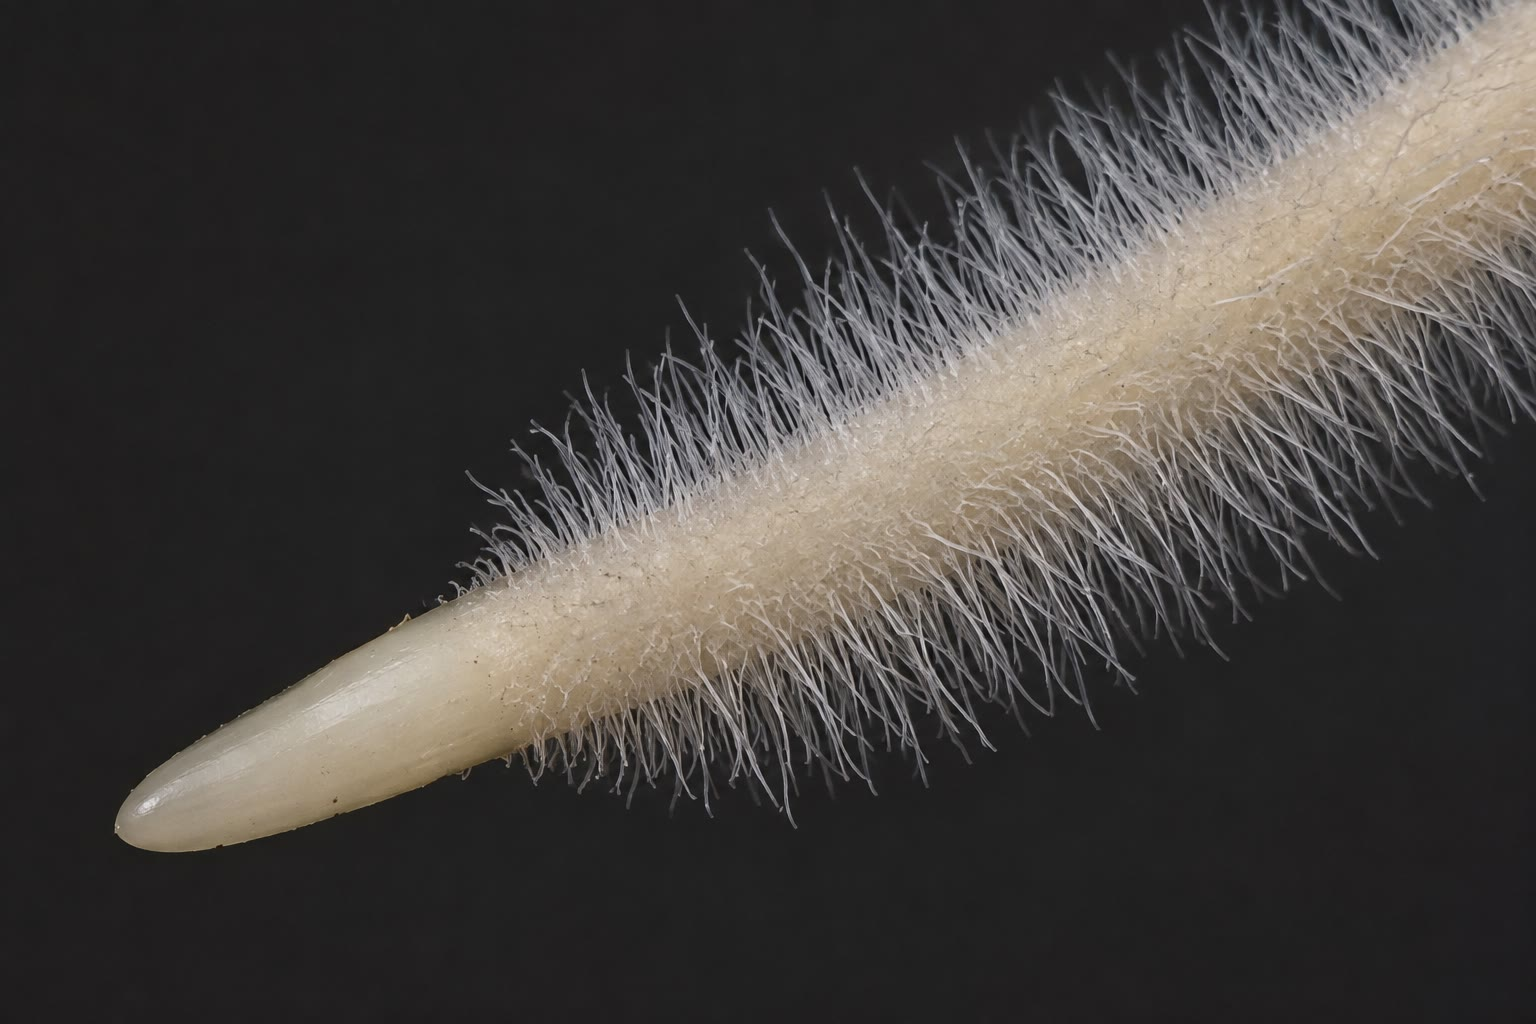
\includegraphics[width=0.58\linewidth]{images/book3/ai/b3-03-root-hairs.jpg}

{\small \omterm{def:b1:flowering-plant-organization:organs}{Pelos radiculares} numa plântula de rabanete, alguns milímetros
atrás da ponta nua. Cada pelo é uma única célula epidérmica crescida
para dentro do solo; juntos, eles multiplicam muitas vezes a superfície
absorvente.}
\end{omfigure}

\begin{example}[As duas superfícies do carvalho]\label{ex:b1:flowering-plant-organization:oaksurfaces}
Um carvalho cuja copa sombreia \qty{100}{m^2} com $L = 5$ carrega
\qty{500}{m^2} de \omterm{def:b1:flowering-plant-organization:organs}{folha}. As raízes finas dele, a alguns quilômetros por
metro cúbico ao longo de \qty{100}{m^3} de solo, oferecem várias
centenas de metros quadrados, e os \omterm{def:b1:flowering-plant-organization:organs}{pelos radiculares} delas, mais um
milhar: a superfície absorvente subterrânea é várias vezes a superfície
fotossintética acima, sobre os mesmos metros quadrados de solo.
\end{example}

\section{Crescimento e forma}

\begin{definition}[Meristemas, crescimento primário e secundário]\label{def:b1:flowering-plant-organization:meristem}
Um \emph{meristema}\index{meristema} é um tecido de células pequenas e
indiferenciadas que continuam se dividindo. Os
\emph{meristemas apicais}\index{meristema apical} nas pontas de cada
\omterm{def:b1:flowering-plant-organization:organs}{caule} e de cada \omterm{def:b1:flowering-plant-organization:organs}{raiz} produzem o
\emph{crescimento primário}\index{crescimento primário}: o alongamento e
os tecidos primários acima. Os
\emph{meristemas laterais}\index{meristema lateral} --- o câmbio
vascular entre o \omterm{def:b1:flowering-plant-organization:tissues}{xilema} e o \omterm{def:b1:flowering-plant-organization:tissues}{floema}, e o felogênio sob a epiderme ---
produzem o
\emph{crescimento secundário}\index{crescimento secundário}: o
espessamento, que acrescenta madeira (\omterm{def:b1:flowering-plant-organization:tissues}{xilema} secundário) para dentro e
casca para fora, nos \omterm{def:b1:flowering-plant-organization:organs}{caules} e nas raízes de árvores e arbustos. Os
mecanismos da atividade meristemática pertencem ao volume do Ano 2.
\end{definition}

\begin{omfigure}
\begin{tikzpicture}[font=\small, >=Stealth, line cap=round]
  % root outline (vertical, tip at bottom)
  \draw[thick, omDef!60!black, fill=omDef!8] (-0.7,5.2) -- (-0.7,1.3) .. controls (-0.7,0.4) and (-0.3,0) .. (0,-0.2) .. controls (0.3,0) and (0.7,0.4) .. (0.7,1.3) -- (0.7,5.2);
  % root cap
  \draw[thick, omDef!60!black, fill=omDef!25] (-0.72,0.9) .. controls (-0.75,0.2) and (-0.3,-0.35) .. (0,-0.45) .. controls (0.3,-0.35) and (0.75,0.2) .. (0.72,0.9) .. controls (0.5,0.55) and (0.2,0.4) .. (0,0.45) .. controls (-0.2,0.4) and (-0.5,0.55) .. (-0.72,0.9);
  % meristem
  \fill[omThm!45] (0,0.95) ellipse (0.45 and 0.35);
  % vascular strand
  \draw[thick, omDef!60!black, fill=omDef!30] (-0.15,5.2) -- (-0.15,1.9) .. controls (-0.1,1.5) .. (0,1.35) .. controls (0.1,1.5) .. (0.15,1.9) -- (0.15,5.2);
  % root hairs
  \foreach \y in {3.4,3.7,4.0,4.3,4.6,4.9} { \draw[omDef!60!black] (-0.7,\y) -- (-1.5,\y+0.15); \draw[omDef!60!black] (0.7,\y) -- (1.5,\y+0.15); }
  % zone brackets
  \draw[thick, gray] (2.0,-0.45) -- (2.2,-0.45) -- (2.2,0.6) -- (2.0,0.6); \node[right, align=left, font=\footnotesize] at (2.3,0.1) {coifa: protege a ponta,\\ percebe a gravidade};
  \draw[thick, gray] (2.0,0.6) -- (2.2,0.6) -- (2.2,1.4) -- (2.0,1.4); \node[right, align=left, font=\footnotesize] at (2.3,1.0) {zona de divisão:\\ meristema apical (vermelho)};
  \draw[thick, gray] (2.0,1.4) -- (2.2,1.4) -- (2.2,3.1) -- (2.0,3.1); \node[right, align=left, font=\footnotesize] at (2.3,2.25) {zona de alongamento: as células\\ se alongam dez vezes, empurrando\\ a ponta pelo solo};
  \draw[thick, gray] (2.0,3.1) -- (2.2,3.1) -- (2.2,5.2) -- (2.0,5.2); \node[right, align=left, font=\footnotesize] at (2.3,4.15) {zona de diferenciação:\\ pelos radiculares, xilema\\ e floema maduros};
  \node[left, font=\footnotesize, align=right] at (-1.6,4.4) {pelos radiculares};
  \node[left, font=\footnotesize, align=right] at (-0.85,2.4) {cilindro\\ vascular\\ em formação};
\end{tikzpicture}

{\small Corte longitudinal de uma ponta de \omterm{def:b1:flowering-plant-organization:organs}{raiz}. Atrás da coifa
protetora, o \omterm{def:b1:flowering-plant-organization:meristem}{meristema apical} se divide; os produtos dele se alongam e
depois se diferenciam nos tecidos da \omterm{def:b1:flowering-plant-organization:organs}{raiz} madura e emitem \omterm{def:b1:flowering-plant-organization:organs}{pelos
radiculares}. Toda a sequência ocupa alguns milímetros e avança à medida
que a \omterm{def:b1:flowering-plant-organization:organs}{raiz} cresce.}
\end{omfigure}

\begin{proposition}[A forma segue o local]\label{prop:b1:flowering-plant-organization:plasticity}
Como o crescimento dela é modular e indeterminado, uma planta molda o
próprio corpo ao local
(\emph{plasticidade fenotípica}\index{plasticidade fenotípica}): uma
árvore crescida em campo aberto ramifica baixo e largo, e a mesma
espécie numa floresta produz um tronco alto e nu; uma planta em solo
seco destina mais do crescimento dela às raízes, e na sombra, mais às
\omterm{def:b1:flowering-plant-organization:organs}{folhas}. As espécies de ambientes secos
(\emph{xerófitas}\index{xerófita}) carregam \omterm{def:b1:flowering-plant-organization:tissues}{cutículas} espessas,
\omterm{def:b1:flowering-plant-organization:tissues}{estômatos} afundados em criptas ou protegidos por pelos, \omterm{def:b1:flowering-plant-organization:organs}{folhas} pequenas
ou suculentas e raízes profundas; as espécies de ambientes úmidos
(\emph{hidrófitas}\index{hidrófita}) carregam \omterm{def:b1:flowering-plant-organization:tissues}{cutículas} finas, \omterm{def:b1:flowering-plant-organization:tissues}{estômatos}
na face superior de \omterm{def:b1:flowering-plant-organization:organs}{folhas} flutuantes, e um tecido cheio de ar
(\emph{aerênquima}\index{aerênquima}) que leva oxigênio até as raízes na
lama anóxica.
\end{proposition}

\begin{example}[Mamífero e planta, lado a lado]\label{ex:b1:flowering-plant-organization:comparison}
Nutrição: o mamífero come matéria orgânica; a planta a fabrica a partir
de dióxido de carbono, água e luz. \omterm{prop:b1:organism-environment:surfaces}{Superfícies de troca}: internas, de
tamanho fixo, irrigadas pelo sangue; externas, crescentes, ventiladas
pelo vento e pelo solo. \omterm{def:b1:organism-environment:milieu}{Meio interno}: um líquido regulado a temperatura
e composição constantes; nenhum --- as células regulam o próprio
conteúdo e a temperatura da planta é a do ar. Crescimento: até uma forma
adulta fixa; aberto e modular, a vida inteira. Movimento: o animal vai
até o alimento; a planta cresce em direção à luz e à água. Coordenação:
nervos e hormônios, em segundos a horas; só hormônios, em horas a dias.
Cada coluna é uma maneira coerente de ser um \omterm{def:b1:organism-environment:organism}{sistema aberto}.
\end{example}

\section{Exercícios}

\begin{exercise}[$\star$]\label{exo:b1:flowering-plant-organization:1}
Cite os três \omterm{def:b1:mammal-organization:organ}{órgãos} vegetativos de uma planta com flores e a função
principal de cada um.
\end{exercise}

\begin{exercise}[$\star$]\label{exo:b1:flowering-plant-organization:2}
Defina um módulo da parte aérea e explique o que significa ``\omterm{prop:b1:flowering-plant-organization:modular}{crescimento
indeterminado}''.
\end{exercise}

\begin{exercise}[$\star$]\label{exo:b1:flowering-plant-organization:3}
Para cada tecido --- epiderme, \omterm{def:b1:flowering-plant-organization:tissues}{parênquima}, \omterm{def:b1:flowering-plant-organization:tissues}{colênquima}, \omterm{def:b1:flowering-plant-organization:tissues}{esclerênquima},
\omterm{def:b1:flowering-plant-organization:tissues}{xilema}, \omterm{def:b1:flowering-plant-organization:tissues}{floema} ---, diga se as células dele estão vivas na maturidade e
o que ele faz.
\end{exercise}

\begin{exercise}[$\star$]\label{exo:b1:flowering-plant-organization:4}
A partir da figura da interceptação de luz, que fração da luz chega ao
solo sob um prado com $L = 3$ e $k = 0.3$, e sob uma floresta de \omterm{def:b1:flowering-plant-organization:organs}{folhas}
largas com $L = 6$ e $k = 0.5$?
\end{exercise}

\begin{exercise}[$\star\star$]\label{exo:b1:flowering-plant-organization:5}
Um corte mostra uma estrela central de \omterm{def:b1:flowering-plant-organization:tissues}{xilema} com quatro braços, \omterm{def:b1:flowering-plant-organization:tissues}{floema}
entre os braços, um anel de células com paredes radiais espessadas em
volta dele, e uma zona larga de células arredondadas do lado de fora.
Identifique o \omterm{def:b1:mammal-organization:organ}{órgão} e o grupo, dando as duas características que decidem
cada um.
\end{exercise}

\begin{exercise}[$\star\star$]\label{exo:b1:flowering-plant-organization:6}
Explique, usando a mecânica de uma viga e a de um cabo, por que o \omterm{def:b1:flowering-plant-organization:tissues}{tecido
vascular} fica num anel periférico no \omterm{def:b1:flowering-plant-organization:organs}{caule} e num cilindro central na
\omterm{def:b1:flowering-plant-organization:organs}{raiz}.
\end{exercise}

\begin{exercise}[$\star\star$]\label{exo:b1:flowering-plant-organization:7}
Uma cultura tem $L = 4$ e $k = 0.6$. Que fração da luz ela intercepta?
Quanto subiria a interceptação se $L$ passasse a 6? Comente o retorno
das \omterm{def:b1:flowering-plant-organization:organs}{folhas} a mais.
\end{exercise}

\begin{exercise}[$\star\star$]\label{exo:b1:flowering-plant-organization:8}
O pé de centeio de Dittmer tinha \qty{623}{km} de raízes e
\qty{240}{m^2} de superfície radicular. Calcule o diâmetro médio das
raízes. Se as \omterm{def:b1:flowering-plant-organization:organs}{folhas} dele somavam \qty{5}{m^2}, qual é a razão entre a
superfície de \omterm{def:b1:flowering-plant-organization:organs}{raiz} mais pelos e a superfície foliar?
\end{exercise}

\begin{exercise}[$\star\star$]\label{exo:b1:flowering-plant-organization:9}
Os \omterm{def:b1:flowering-plant-organization:organs}{pelos radiculares} têm $\qty{10}{\micro m}$ de largura e
$\qty{0.8}{mm}$ de comprimento, a \qty{250}{} por milímetro de \omterm{def:b1:flowering-plant-organization:organs}{raiz}. Por
qual fator eles multiplicam a superfície de uma \omterm{def:b1:flowering-plant-organization:organs}{raiz} de
$\qty{0.4}{mm}$ de diâmetro?
\end{exercise}

\begin{exercise}[$\star\star\star$]\label{exo:b1:flowering-plant-organization:10}
Uma árvore numa floresta tem um tronco nu de \qty{20}{m} e uma copa
pequena; a mesma espécie num campo é larga e ramificada desde
\qty{2}{m}. Explique as duas formas a partir do \omterm{prop:b1:flowering-plant-organization:modular}{crescimento modular} e do
destino das gemas axilares na sombra e na luz, e diga o que essa
plasticidade custa e o que ela rende.
\end{exercise}

\begin{exercise}[$\star\star\star$]\label{exo:b1:flowering-plant-organization:11}
Uma \omterm{prop:b1:flowering-plant-organization:plasticity}{xerófita} tem os \omterm{def:b1:flowering-plant-organization:tissues}{estômatos} afundados em criptas revestidas de pelos.
Explique o que isso faz com o gradiente de vapor de água entre os
espaços de ar da \omterm{def:b1:flowering-plant-organization:organs}{folha} e o vento, e o que isso custa na captação de
dióxido de carbono. Por que essa é uma boa troca num deserto e uma má
troca numa floresta tropical úmida?
\end{exercise}

\begin{exercise}[$\star\star\star$]\label{exo:b1:flowering-plant-organization:12}
``Uma planta não tem \omterm{def:b1:organism-environment:milieu}{meio interno}.'' Discuta em um parágrafo: o que
falta à planta que o mamífero tem, o que as células dela enfrentam em
consequência, e o que ela faz no lugar --- superfícies, crescimento e a
regulação que ela de fato exerce.
\end{exercise}

\section{Problema: As superfícies de um carvalho}

\begin{problem}[{Problema de fim de semana --- as folhas de um carvalho
contadas por área, os estômatos aos bilhões, o carbono e a água aos
quilogramas, e as raízes aos quilômetros, terminando na superfície de
troca que ele espalha sobre cada metro quadrado do seu solo}]
\label{pb:b1:flowering-plant-organization:1}
A copa de um carvalho sombreia \qty{100}{m^2} de solo com um \omterm{def:b1:flowering-plant-organization:lai}{índice de
área foliar} $L = 5$ e um coeficiente de extinção $k = 0.5$. As faces
inferiores das \omterm{def:b1:flowering-plant-organization:organs}{folhas} dele carregam \qty{150}{} \omterm{def:b1:flowering-plant-organization:tissues}{estômatos} por milímetro
quadrado; um poro estomático aberto mede \qty{10}{\micro m} por
\qty{5}{\micro m}. Em média sobre todo o dossel e sobre um dia de
\qty{12}{h}, cada metro quadrado de \omterm{def:b1:flowering-plant-organization:organs}{folha} capta \qty{4}{\micro mol} de
$\mathrm{CO_2}$ e perde \qty{1}{mmol} de vapor de água por segundo. As
raízes finas (diâmetro \qty{0.5}{mm}) correm a \qty{5}{km} por metro
cúbico ao longo de \qty{1}{m} de profundidade de solo sob a copa; os
\omterm{def:b1:flowering-plant-organization:organs}{pelos radiculares} (\qty{10}{\micro m} por \qty{0.5}{mm}) crescem a
\qty{200}{} por milímetro de \omterm{def:b1:flowering-plant-organization:organs}{raiz} fina. Massas molares:
$\mathrm{CO_2}$ \qty{44}{g/mol}, C \qty{12}{g/mol},
$\mathrm{H_2O}$ \qty{18}{g/mol}.

\medskip
\noindent\textbf{Parte I --- \omterm{def:b1:flowering-plant-organization:organs}{Folhas} e luz.}
\begin{enumerate}
  \item Calcule a área foliar total de uma só face da copa.
  \item Calcule a fração da luz que chega ao solo e a fração
        interceptada.
  \item Calcule a fração interceptada se o carvalho tivesse apenas
        $L = 2$, e se tivesse $L = 8$.
  \item Explique, a partir desses números, por que um carvalho para em
        $L \approx 5$.
  \item A \omterm{def:b1:flowering-plant-organization:organs}{folha} média tem \qty{50}{cm^2}. Quantas \omterm{def:b1:flowering-plant-organization:organs}{folhas} a copa carrega?
\end{enumerate}

\medskip
\noindent\textbf{Parte II --- \omterm{def:b1:flowering-plant-organization:tissues}{Estômatos} e carbono.}
\begin{enumerate}[resume]
  \item Calcule o número de \omterm{def:b1:flowering-plant-organization:tissues}{estômatos} da copa.
  \item Calcule a área de um poro aberto e a fração da face inferior das
        \omterm{def:b1:flowering-plant-organization:organs}{folhas} que os poros abertos representam.
  \item Calcule a captação de $\mathrm{CO_2}$ pela copa em mols por
        segundo e em gramas por segundo.
  \item Calcule o $\mathrm{CO_2}$ captado em um dia de \qty{12}{h}, em
        quilogramas, e o carbono que ele contém.
  \item Ao longo de uma estação de crescimento de \qty{150}{} dias,
        quanto carbono a copa fixa? Se metade for respirada pela própria
        árvore, que massa de madeira (\qty{50}{\%} de carbono) ela pode
        acrescentar?
\end{enumerate}

\medskip
\noindent\textbf{Parte III --- Água.}
\begin{enumerate}[resume]
  \item Calcule a água perdida pela copa em mols e em gramas por
        segundo.
  \item Calcule a perda diária de água em litros.
  \item Calcule a razão entre as moléculas de água perdidas e as
        moléculas de $\mathrm{CO_2}$ ganhas. Por que ela é tão grande?
  \item Uma chuva de \qty{2}{mm} cai sobre os \qty{100}{m^2}. Quantos
        dias de transpiração ela cobre, se toda ela chegar às raízes?
\end{enumerate}

\medskip
\noindent\textbf{Parte IV --- Raízes.}
\begin{enumerate}[resume]
  \item Calcule o volume de solo explorado e o comprimento total das
        raízes finas.
  \item Calcule a superfície das raízes finas (cilindros).
  \item Calcule o número de \omterm{def:b1:flowering-plant-organization:organs}{pelos radiculares}.
  \item Calcule a superfície dos \omterm{def:b1:flowering-plant-organization:organs}{pelos radiculares}.
  \item Calcule a superfície absorvente total no subsolo e a razão dela
        com a área foliar de uma só face.
  \item As raízes finas estão a menos de \qty{1}{mm} de que fração do
        volume de solo? (Tome cada \omterm{def:b1:flowering-plant-organization:organs}{raiz} como o eixo de um cilindro de
        raio \qty{1}{mm}.)
  \item Compare com o pé de centeio do capítulo (\qty{620}{km} de raízes
        em \qty{0.05}{m^3}): qual das duas plantas explora o solo dela
        mais a fundo, e por qual fator?
  \item Some a superfície foliar das duas faces e a superfície
        radicular. Divida pelos \qty{100}{m^2} de solo.
  \item Compare isso com a razão, para um ser humano, entre as
        \omterm{prop:b1:organism-environment:surfaces}{superfícies de troca} dobradas (\qty{130}{m^2}) e a superfície
        externa (\qty{2}{m^2}).
  \item Explique em duas frases por que a razão da planta pode continuar
        subindo ao longo da vida dela e a do mamífero não pode.
  \item Enuncie o resultado: a \omterm{prop:b1:organism-environment:surfaces}{superfície de troca} que um carvalho
        espalha por metro quadrado do solo dele, acima e abaixo, em
        metros quadrados.
\end{enumerate}
\end{problem}
